\documentclass[12pt, titlepage]{article}

\usepackage{fullpage}
\usepackage[round]{natbib}
\usepackage{multirow}
\usepackage{booktabs}
\usepackage{tabularx}
\usepackage{graphicx}
\usepackage{float}
\usepackage{hyperref}
\usepackage[dvipsnames]{xcolor}

\hypersetup{
    colorlinks,
    citecolor=black,
    filecolor=black,
    linkcolor=red,
    urlcolor=blue
}
\usepackage[round]{natbib}

\newcounter{acnum}
\newcommand{\actheacnum}{AC\theacnum}
\newcommand{\acref}[1]{AC\ref{#1}}

\newcounter{ucnum}
\newcommand{\uctheucnum}{UC\theucnum}
\newcommand{\uref}[1]{UC\ref{#1}}

\newcounter{mnum}
\newcommand{\mthemnum}{M\themnum}
\newcommand{\mref}[1]{M\ref{#1}}

\title{SE 3XA3: Software Requirements Specification\\Legend of Python}

\author{Group \# 1, Lava Boys Inc.
    \\ Bilal Jaffry, affryb
    \\ Giacomo Loparco, loparcog
    \\ Lucas Zacharewicz, zacharel
}

\date{\today}


\begin{document}

\maketitle

\pagenumbering{roman}
\tableofcontents
\listoftables
\listoffigures
\begin{table}[hbp]
\caption{\bf Revision History}
\begin{tabularx}{\textwidth}{p{3cm}p{2cm}X}
\toprule {\bf Date} & {\bf Version} & {\bf Notes}\\
\midrule
November 7th & 1.0 & Started the Document\\
November 9th & 1.1 & Finished the Document\\
December 3rd & 1.2 & Rev 1 Update\\
\bottomrule
\end{tabularx}
\end{table}


\newpage

\pagenumbering{arabic}

\section{Introduction}
\subsection{Overview}
The Legend of Python projects purpose is to create a re-implementation of a open-source project for the original The Legend of Zelda, released in 1986 for the Nintendo Entertainment System video-game console. This project will allow a user to control the player character, while exploring several designed levels.
\subsection{Context}
This Module Guide's purpose is to provide a modular decomposition of the Legend of Python project. This document also provides a look into the modular structure of the project and how each of these modules collectively meet the functional and non-functional requirements for system, outlined in the Software Requirements Specification. This document is supplemented by the presence of the Module Interface Specification, providing information for all the program syntax and the semantics regarding each module and its respective methods. 
\subsection{Design Principles}
The design principles utilized in the development of this project and displayed in this Module Guide are the properties of Encapsulation, Information Hiding and that of the Uses Relation Hierarchy.
The Uses Relation Hierarchy should have no cycles, ensuring efficient and independent software design. Module's that both rely on each other should not be present, and the system should follow the low coupling and high cohesion principle. This principle would ensure the system and its module components are related strongly. Information Hiding for the project hides the process in how each module works in the system when acted upon by the user. Finally, the principle of Encapsulation is to be followed allowing for changes in the implementation of a module but not the interface the module is used in.
\subsection{Document Structure}
The following Module Guide is as follows:
\begin{description}
\item[$\bullet$ 2]Anticipated and Unlikely Changes affecting the system. 
\item[$\bullet$ 3] Module Hierarchy, detailing all the modules and the hierarchy, categorizing each module in their respective categories of Hardware/Behaviour/Software hiding.
\item[$\bullet$ 4] Connection Between Requirements and Design, detailing how each module satisfies the requirements of the software.
\item[$\bullet$ 5] Module Decomposition, providing the module, which component of Hardware/Behaviour/Software hiding it is a member of, and what function each module accomplishes in the entire system.
\item[$\bullet$ 6] Traceability Matrix, providing the association of the requirements of the software system to the modules implemented, as well as the matrix representing the trace back for modules affected by the the anticipated changes.
\item[$\bullet$ 7] Uses Hierarchy, providing the uses relations between each  of the modules.
\end{description}





\section{Anticipated and Unlikely Changes} \label{SecChange}

\subsection{Anticipated Changes} \label{SecAchange}
This section will display the likely changes the software system will encounter during its use and distribution.

\begin{description}
    \item[\refstepcounter{acnum} \actheacnum \label{AC1}:] The data structure implementation of the various levels of the system.
    \item[\refstepcounter{acnum} \actheacnum \label{AC2}:] Structure of display elements in User Interface through the Heads Up Display.
    \item[\refstepcounter{acnum} \actheacnum \label{AC3}:] Basic NPC enemy placement in individual rooms.
    \item[\refstepcounter{acnum} \actheacnum \label{AC4}:] Level transitions collision trigger for user movement.
    \item[\refstepcounter{acnum} \actheacnum \label{AC5}:] Font rendering class will change its inheritance from Pygame Sprite object to Font object.
\end{description}

\subsection{Unlikely Changes} \label{SecUchange}

\begin{description}
\item[\refstepcounter{ucnum} \uctheucnum \label{UC1}:] Input/Output devices to control the user player. The system will only respond to keyboard input and output using the available display devices.
\item[\refstepcounter{ucnum} \uctheucnum \label{UC2}:] The height/width for the output window and Heads Up Display.
\item[\refstepcounter{ucnum} \uctheucnum \label{UC3}:] The NPC enemy movement and attack logic .
\item[\refstepcounter{ucnum} \uctheucnum \label{UC4}:] Spritesheets for the player, enemy, items, and dungeon. 
\end{description}

\section{Module Hierarchy} \label{SecMH}

This section provides an overview of the module design. Modules are summarized
in a hierarchy decomposed by secrets in Table \ref{TblMH}. The modules listed
below, which are leaves in the hierarchy tree, are the modules that will
actually be implemented.

\begin{description}
\item [\refstepcounter{mnum} \mthemnum \label{mHH}:] Aquamentus
\item [\refstepcounter{mnum} \mthemnum \label{mHH}:] Boomerang
\item [\refstepcounter{mnum} \mthemnum \label{mHH}:] Boss
\item [\refstepcounter{mnum} \mthemnum \label{mHH}:] Constants data
\item [\refstepcounter{mnum} \mthemnum \label{mHH}:] Enemy
\item [\refstepcounter{mnum} \mthemnum \label{mHH}:] Fireball
\item [\refstepcounter{mnum} \mthemnum \label{mHH}:] Health Bar
\item [\refstepcounter{mnum} \mthemnum \label{mHH}:] Item
\item [\refstepcounter{mnum} \mthemnum \label{mHH}:] Keese
\item [\refstepcounter{mnum} \mthemnum \label{mHH}:] Player
\item [\refstepcounter{mnum} \mthemnum \label{mHH}:] Render Font
\item [\refstepcounter{mnum} \mthemnum \label{mHH}:] Rupee
\item [\refstepcounter{mnum} \mthemnum \label{mHH}:] Sprite Sheet
\item [\refstepcounter{mnum} \mthemnum \label{mHH}:] Stalfos
\item [\refstepcounter{mnum} \mthemnum \label{mHH}:] Sword
\item [\refstepcounter{mnum} \mthemnum \label{mHH}:] Door
\item [\refstepcounter{mnum} \mthemnum \label{mHH}:] Level
\item [\refstepcounter{mnum} \mthemnum \label{mHH}:] Level Data
\item [\refstepcounter{mnum} \mthemnum \label{mHH}:] Level Manager
\item [\refstepcounter{mnum} \mthemnum \label{mHH}:] Wall
\item [\refstepcounter{mnum} \mthemnum \label{mHH}:] Colour Data
\item [\refstepcounter{mnum} \mthemnum \label{mHH}:] Window Data
\item [\refstepcounter{mnum} \mthemnum \label{mHH}:] Main Run File
\item [\refstepcounter{mnum} \mthemnum \label{mHH}:] Block
\item [\refstepcounter{mnum} \mthemnum \label{mHH}:] Key
\end{description}


\begin{table}[h!]
\centering
\begin{tabular}{p{0.3\textwidth} p{0.6\textwidth}}
\toprule
\textbf{Level 1} & \textbf{Level 2}\\
\midrule

\multirow{7}{0.3\textwidth}{Behaviour-Hiding Module}
& Aquamentus \\
& Boomerang \\
& Fireball \\
& Health Bar \\
& Item \\
& Keese \\
& Player \\
& Rupee \\
& Stalfos \\
& Sword \\
& Door \\
& Level \\
& Level Manager \\
& Wall \\
& Block \\
\midrule

\multirow{3}{0.3\textwidth}{Software Decision Module}
& Boss \\
& Colour Data \\
& Constants data \\
& Enemy \\
& Level Data \\
& Main Run File \\
& Render Font \\
& Sprite Sheet \\
& Window Data \\
\bottomrule

\end{tabular}
\caption{Module Hierarchy}
\label{TblMH}
\end{table}

\section{Connection Between Requirements and Design} \label{SecConnection}
The design of the system was designed to satisfy all the requirements specified in the SRS (Software Requirements Specification). The python module Main Run File is the class that consolidates all the components of the game system is the file ran when using the custom makefile for the system.  The Player module of the system controls the player character movement, satisfying with the Look and Feel/Usability requirements of the system, ensuring that the movement and attack animations are accurate to the original release. The controllable player character responds accurately and consistently to users keyboard inputs.The input parameters of the system are also satisfied, with the [W,A,S,D] keyboard keys initialized for movement of the player character. The system does not interfere with any other processes running on the given system, as well as ensuring the system interacts with the respective Operating System properly.

The Sprite Sheet module and the  accurately renders sprites to screen without unforeseen rendering issues, satisfying the Performance Requirements of the system, ensuring the various sprites are render precisely and consistently at a 60 Hz refresh rat. The eventual collective file size further supports the Performance Requirements of the software project ensuring the collective file size of the system is under the 500MB limit. In order to effectively design the software system to ensure the Maintainability and Support Requirements were met, the file paths for the various file used in the system, such as sprites in the Sprite Sheet module and the fonts in the Render Font module, the system was designed to run with local directory based on the Python OS library. This library guaranteed the software can be compiled on  various Operating Systems (Windows/Linux) without any possible issues. 

The resultant software is kept simple and concise for users to interact with, allowing for users to access and modify this open source software with ease. The design of the software reliably follows all aspects of the original, both culturally and legally, ensuring no Cultural and Legal requirements are violated. The design of the system does not compromise the users data during or after run-time of the software ensuring the Health and Safety Requirements of the system are met consistently.
\section{Module Decomposition} \label{SecMD}

Modules are decomposed according to the principle of ``information hiding''
proposed by \citet{ParnasEtAl1984}. The \emph{Secrets} field in a module
decomposition is a brief statement of the design decision hidden by the
module. The \emph{Services} field specifies \emph{what} the module will do
without documenting \emph{how} to do it. For each module, a suggestion for the
implementing software is given under the \emph{Implemented By} title. If the
entry is \emph{OS}, this means that the module is provided by the operating
system or by standard programming language libraries.  Also indicate if the
module will be implemented specifically for the software.

\subsection{Behaviour-Hiding Module}

\begin{description}
\item[Secrets:] Behaviours
\item[Services:] Describes the visible behaviour of the game. Acts as the interpreter between the Hardware Hiding Module and the Software Decision Module.
\item[Implemented By:] N/A
\end{description}

\subsubsection{Aquamentus Module}

\begin{description}
\item[Secrets:] \textcolor{blue}{How Aquamentus moves and attacks.}
\item[Services:] Controls the boss enemy Aquamentus in the game.
\item[Implemented By:] Aquamentus
\end{description}

\subsubsection{Block}

\begin{description}
	\item[Secrets:] \textcolor{blue}{Block creation and collision detection}
	\item[Services:] \textcolor{blue}{Provides collectible blocks within dungeon levels, accepting any argument of sprite}
	\item[Implemented By:] \textcolor{blue}{Block}
\end{description}

\subsubsection{Boomerang}

\begin{description}
  \item[Secrets:] \textcolor{blue}{Boomerang movement and hitbox.}
  \item[Services:] Controls the movement of the in game item boomerang.
  \item[Implemented By:] Boomerang
  \end{description}

\subsubsection{Fireball}

\begin{description}
  \item[Secrets:] \textcolor{blue}{Fireball movement and hitbox.}
  \item[Services:] Controls the fireball projectiles in the game. 
  \item[Implemented By:] Fireball
\end{description}

\subsubsection{Health Bar}

\begin{description}
  \item[Secrets:] \textcolor{blue}{Health bar rendering.}
  \item[Services:] Provides the in game health bar for the player.
  \item[Implemented By:] Health Bar
\end{description}

\subsubsection{Item}

\begin{description}
  \item[Secrets:] \textcolor{blue}{Item creation, rendering, and behaviour.}
  \item[Services:] Provides the in game collectible items.
  \item[Implemented By:] Item
\end{description}

\subsubsection{Keese}

\begin{description}
  \item[Secrets:] \textcolor{blue}{Keese movement and animation.}
  \item[Services:] Controls the Keese enemies behaviour in the game.
  \item[Implemented By:] Keese
\end{description}

\subsubsection{Player}

\begin{description}
  \item[Secrets:] \textcolor{blue}{Player's actions and animations.}
  \item[Services:] Provides the player movement and actions for controlling the character in game.
  \item[Implemented By:] Player
\end{description}

\subsubsection{Rupee}

\begin{description}
  \item[Secrets:] \textcolor{blue}{Rupee rendering and behaviour.}
  \item[Services:] Provides the rupee item in the game
  \item[Implemented By:] Rupee
\end{description}

\subsubsection{Stalfos}

\begin{description}
  \item[Secrets:] \textcolor{blue}{Stalfos movement and animation.}
  \item[Services:] Controls the Stalfos enemies in the game. 
  \item[Implemented By:] Stalfos
\end{description}

\subsubsection{Sword}

\begin{description}
  \item[Secrets:] \textcolor{blue}{Sword collision and actions.}
  \item[Services:] Provides the sword attack for the player.
  \item[Implemented By:] Sword
\end{description}

\subsubsection{Door}

\begin{description}
  \item[Secrets:] \textcolor{blue}{Door behaviour and rendering.}
  \item[Services:] Allows for the use of doors to traverse the map.
  \item[Implemented By:] Door
\end{description}

\subsubsection{Level}

\begin{description}
  \item[Secrets:] \textcolor{blue}{Level creation and rendering.}
  \item[Services:] Allows for rooms on the map to be created.
  \item[Implemented By:] Level
\end{description}

\subsubsection{Level Manager}

\begin{description}
  \item[Secrets:] \textcolor{blue}{Map creation and transition behaviour.}
  \item[Services:] Allows for rooms to be linked together to make full maps. 
  \item[Implemented By:] Level Manager
\end{description}

\subsubsection{Wall}

\begin{description}
  \item[Secrets:] \textcolor{blue}{Wall creation and collision detection.}
  \item[Services:] Provides collidable walls in the game.
  \item[Implemented By:] Wall
\end{description}

\subsection{Software Decision Module}

\begin{description}
\item[Secrets:] \textcolor{blue}{Data structures.}
\item[Services:] The base data structures that model the game's back end. 
\item[Implemented By:] Pygame
\end{description}

\subsubsection{Boss}

\begin{description}
  \item[Secrets:] \textcolor{blue}{Boss framework and initialization.}
  \item[Services:] Provides a bare bones boss game loop to build upon
  \item[Implemented By:] Boss
\end{description}

\subsubsection{Colour Data}

\begin{description}
  \item[Secrets:] \textcolor{blue}{Colour constants.}
  \item[Services:] Provides colour constants for the game.
  \item[Implemented By:] Colour Data
\end{description}

\subsubsection{Constants Data}

\begin{description}
  \item[Secrets:] \textcolor{blue}{Constants Data.}
  \item[Services:] Provides the constants for the majority of game variables.
  \item[Implemented By:] Constants Data
\end{description}

\subsubsection{Enemy}

\begin{description}
  \item[Secrets:] \textcolor{blue}{Enemy initialization and framework.}
  \item[Services:] Provides a bare bones implementation of an enemy game loop
  \item[Implemented By:] Enemy
\end{description}

\subsubsection{Level Data}

\begin{description}
  \item[Secrets:] \textcolor{blue}{Data for level creation.}
  \item[Services:] Provides the level data for all the rooms on the map.
  \item[Implemented By:] Level Data
\end{description}

\subsubsection{Main Run File}

\begin{description}
  \item[Secrets:] \textcolor{blue}{Main game loop.}
  \item[Services:] Main game loop, \textcolor{blue}{running other modules and producing sounds for the game.}
  \item[Implemented By:] Main Run File
\end{description}

\subsubsection{Render Font}

\begin{description}
  \item[Secrets:] \textcolor{blue}{How font is rendered.}
  \item[Services:] Renders onscreen font.
  \item[Implemented By:] Pygame, Render Font
\end{description}

\subsubsection{Sprite Sheet}

\begin{description}
  \item[Secrets:] \textcolor{blue}{Sprite Sheet parsing.}
  \item[Services:] Provides spritesheet image grabbing for onscreen graphics
  \item[Implemented By:] Pygame, Sprite Sheet
\end{description}

\subsubsection{Window Data}

\begin{description}
  \item[Secrets:] \textcolor{blue}{Window constants.}
  \item[Services:] Provides the constants for the window of the game.
  \item[Implemented By:] Window Data 
\end{description}

\section{Traceability Matrix} \label{SecTM}

% the table should use mref, the requirements should be named, use something
% like fref
\begin{table}[H]
\centering
\begin{tabular}{p{0.2\textwidth} p{0.6\textwidth}}
\toprule
\textbf{F Req.} & \textbf{Modules}\\
\midrule
FR1 & M23\\
FR2 & M23\\
FR3 & M23\\
FR4 & \textcolor{blue}{M23}\\
FR5 & \textcolor{blue}{M18, M19}\\
FR6 & \textcolor{blue}{M18, M19}\\
FR7 & \textcolor{blue}{M20, M24}\\
FR8 & \textcolor{blue}{M8, M10}\\
FR9 & \textcolor{blue}{M8}\\
FR10 & \textcolor{blue}{M2, M10}\\
FR11 & \textcolor{blue}{M12, M25}\\
FR12 & \textcolor{blue}{M4, M10}\\
FR13 & \textcolor{blue}{M10, M23}\\
FR14 & \textcolor{blue}{M1, M9, M14}\\
FR15 & \textcolor{blue}{M1, M3, M5, M9, M14}\\
FR16 & \textcolor{blue}{M4, M9, M14}\\
FR17 & \textcolor{blue}{M1, M3, M5, M9, M10, M14}\\
FR18 & \textcolor{blue}{M3, M5, M10}\\
FR19 & \textcolor{blue}{M10, M23}\\
FR20 & \textcolor{blue}{M8, M9, M14, M19}\\
FR21 & \textcolor{blue}{M8}\\
FR22 & \textcolor{blue}{M8, M10}\\
FR23 & \textcolor{blue}{M8, M10}\\
FR24 & \textcolor{blue}{M10, M16}\\
FR25 & \textcolor{blue}{M23}\\
FR26 & \textcolor{blue}{M8, M10, M23}\\
FR27 & \textcolor{blue}{M8, M10, M18, M19}\\
\bottomrule
\end{tabular}
\caption{Trace Between Functional Requirements and Modules}
\label{TblRT}
\end{table}

\begin{table}[H]
\centering
\begin{tabular}{p{0.2\textwidth} p{0.6\textwidth}}
\toprule
\textbf{N-F Req.} & \textbf{Modules}\\
\midrule
NFR1 & M1, M3, M5, M9, M10, M14, M19, M23\\
NFR2 & M23\\
NFR3 & M22, M23\\
NFR4 & \textcolor{blue}{M19, M23}\\
NFR5 & M1, M2, M9, M19, M13, M14, M15, M16, M17, M20\\
NFR6 & M10, M23\\
NFR7 & M23\\
NFR8 & N/A\\
NFR9 & M*\\
NFR10 & M10, M23\\
NFR11 & M22, M23\\
NFR12 & N/A\\
NFR13 & N/A\\
NFR14 & N/A\\
NFR15 & N/A\\
NFR16 & N/A\\
NFR17 & N/A\\
NFR18 & N/A\\
NFR19 & M13, M19\\
NFR20 & N/A\\
NFR21 & N/A\\
NFR22 & N/A\\
NFR23 & N/A\\
NFR24 & N/A\\
\bottomrule
\end{tabular}
\caption{Trace Between Non-Functional Requirements and Modules}
\label{TblRT}
\end{table}

\begin{table}[H]
\centering
\begin{tabular}{p{0.2\textwidth} p{0.6\textwidth}}
\toprule
\textbf{AC} & \textbf{Modules}\\
\midrule
AC1 & M18, M19 \\
AC2 & M7, M11, M12 \\
AC3 & M2, M3, M5 \\
AC4 & M1, M3, M18 \\
AC5 & M18 \\
AC6 & M10, M16, M19 \\
AC7 & M11 \\
\bottomrule
\end{tabular}
\caption{Trace Between Anticipated Changes and Modules}
\label{TblACT}
\end{table}

\section{Use Hierarchy Between Modules} \label{SecUse}

\begin{figure}[H]
\centering
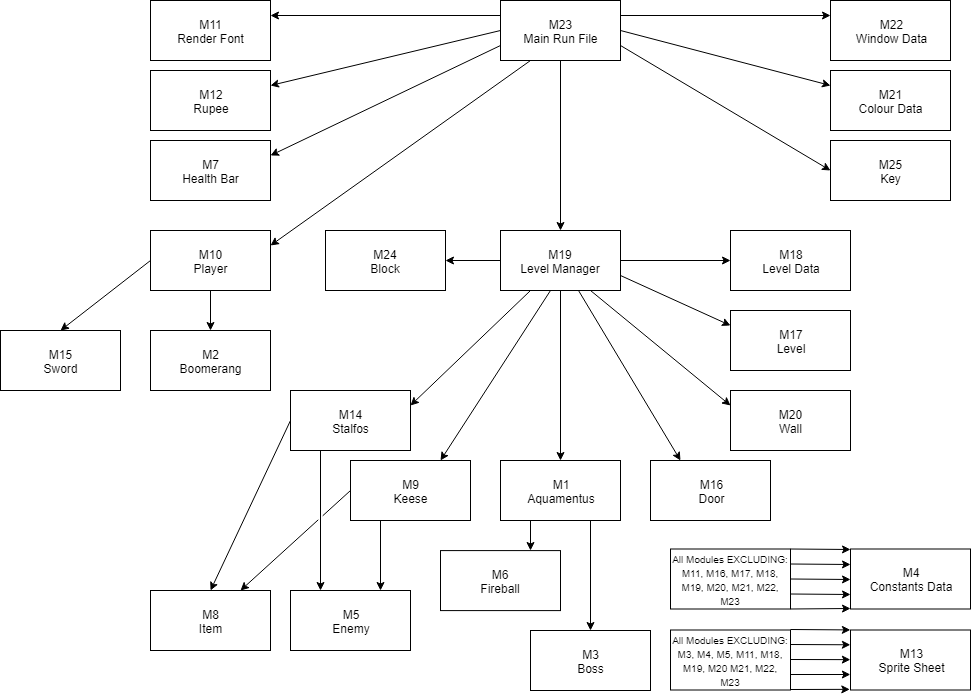
\includegraphics[width=1\textwidth]{MGOG.png}
\caption{Use hierarchy among modules}
\label{FigUH}
\end{figure}

%\section*{References}

\bibliographystyle {plainnat}
\bibliography {MG}

\end{document}